\section{Methodology}
In this section, the methodology utilized for the research will be provided. A diagram showing all the steps in the methodology is provided in the next page. The primary purpose of this research is to assess the effect of dietary patterns on the cause (ACR - Albumin Creatinine Ratio) as well as the mortality and survival in relation to chronic kidney disease (CKD)/End Stage Renal Disease (ESRD). A dataset released by CDC/Health.gov with the dietary habits and a CKD measure named Albumin Creatinine Ratio (ACR) of around 10,000 individuals are studied. Also, age group based mortality and survival of CKD/ESRD patients provided by USRDS are studied. Afterwards, utilized Principal Component Analysis to identify the most important food groups and subgroups affecting the ACR value and the Mortality/Survival then utilized Statistical Regression and Factor analysis to understand the correlation of ACR, and Mortality/Survival to dietary patterns. Machine learning approaches such as Regression, Polynomial Regression, and Bayesian with or without 10 fold cross validations are applied on the datasets to understand if dietary patterns can be used to predict ACR values and mortality. The experiments showed 57 to 95\% accuracy in the test data depending on the methodology applied. 

\noindent Additionally, dietary recommendations as provided by health.gov are utilized for food groups/subgroups. Association of CKD mortality and ACR values with deviation from the recommended amount is studied. Another study [11] on shifting from current recommendations conducted by health.gov is explored. Will the recommended shift [11] from current diet style [15] can have an improved outcome or not is also explored (optional goal).

\noindent \textbf{Study Selection}

\medskip 

\noindent For dietary patterns, CKD measures (such as Albumin Creatinine Ratio - ACR) , and Kidney condition measures, a dataset from the National Health and Nutrition Examination Survey on dietary habits conducted by the Centers for Disease Control and Prevention (CDC) [10] was used. The survey has data from 1996 to 2016 [10]. This study primarily utilized data for 2015-2016. The survey recorded 24 hours individual food item intake amount. Two surveys were taken within 3 to 10 days apart. Each survey provided food item intake amount in a day, also mentioned the diet style, and diet-restrictions. Individual food items are represented using USDA food code. The survey also provided total nutrients data. CDC also released examination, laboratory, demographics, and other related data for those participants.

\medskip 
\noindent For mortality and survival information, dataset from the United States Renal Data System (USRDS) on CKD and ESRD [16, 17] was utilized. “USRDS investigates the transition of care from CKD to ESRD and end-of-life care for those with advanced kidney disease” [19]. USRDS also releases data on the Incidence, Prevalence, Patient Characteristics, and Treatment Modalities on CKD, and ESRD patients. USRDS reports the survival and mortality using metrics such as Mortality rates: ESRD patients,  Mortality rates: Dialysis patients, Total Mortality Count, 90 day survival for dialysis and/or transplantation patients, 10 year survival for dialysis and/or transplantation patients, Avg. Expected remaining lifetime with or without pre-condition and treatment options used. The data are either aggregated or patient specific detail data. However, only aggregated data are public where patient specific data access requires special request and permission. This research utilized only the public dataset.

\begin{center}
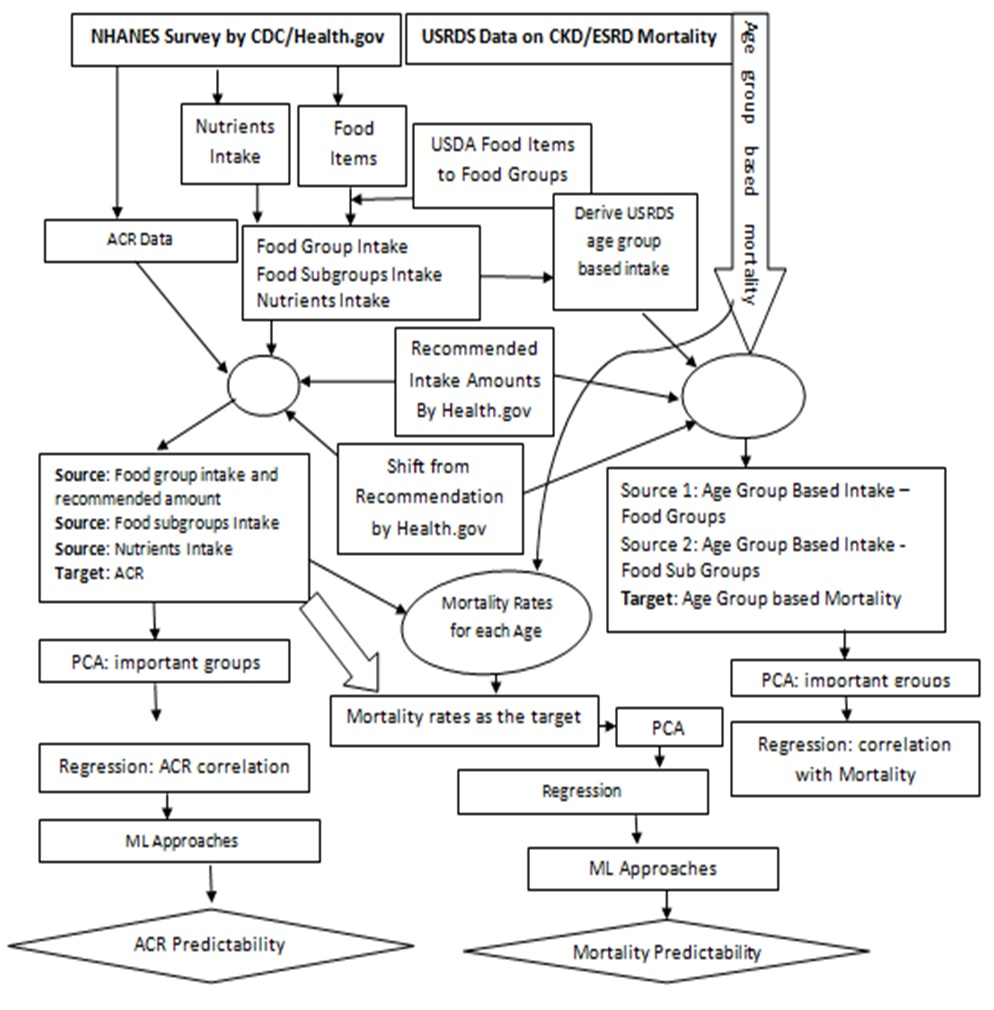
\includegraphics[scale=0.5]{methodology}
\end{center}



\medskip 
\noindent The dietary survey data (NHANES) represented the food items taken by the participants using USDA food codes [14, 12, 13]. Hence, USDA food codes [14, 12, 13] are used to assign food groups and subgroups to the NHANES [10] survey data to properly group/subgroup the dietary intake of the participants with some customizations as provided in the appendix.

\medskip 
\noindent \textbf{Data Synthesis}

\noindent NHANES survey data as provided for two days are averaged to get the intake amount for one day. Both individual food item data and nutrients intake data are averaged. USDA food codes are used to map food items to food groups and subgroups.

\medskip 
\noindent ACR and Kidney condition data for each individual are merged with the averaged food group/subgroup and nutrients data. ACR values are used as the target variable for couple of experiments and study. With this data food group recommendations from health.gov were also merged. This dataset was used for ACR association study. 

\medskip 
\noindent For one mortality/survival study mortality rates from USRDS for each age were merged with the above data. Mortality/survival is used as the target variable.

\medskip 
\noindent For both of the above cases, Principal Component Analysis (PCA) was applied to find out important food groups and subgroups. Afterwards, Regression was applied to find association with ACR and Mortality. Afterwards, Machine Learning approaches such as Linear Regression, Polynomial Regression, Random Forest Regression, Bayesian prediction with or without 10 fold cross validations were applied to study the predictability of ACR Values and Mortality in the test dataset. Test dataset was also part of the above datasets.

\medskip
\noindent For another mortality/survival study, the above synthesized datasets were aggregated for USRDS age groups to calculate average food group/subgroup intake by age groups. With that aggregation mortality/survival data were merged. Mortality/survival is used as the target variable. For this, PCA and Regression were used to find association between food groups and CKD/ESRD mortality
